\documentclass{beamer}

% Theme and Color Scheme
\usetheme{Boadilla}
\usecolortheme{seahorse}
\setbeamersize{text margin left=0.5cm, text margin right=0.5cm}
\setbeamertemplate{footline}{} % Remove footer
\date{}

% Required Packages
\usepackage{graphicx} % For including images
\usepackage{amsmath}  % For advanced math environments
\usepackage{amssymb}
\usepackage{booktabs} % For professional tables
\usepackage[numbers,sort&compress]{natbib} % For citations
\usepackage{qrcode} % For QR codes

% Title Page Information
\title[RMSTSS]{RMSTSS: A Comprehensive Software Suite for Power and Sample Size Calculation in Modern Clinical Trials}
\author{Arnab Aich}
\institute{Florida State University}
\date{\today}

\begin{document}

% Frame 1: Title Page
\begin{frame}
  \titlepage
\end{frame}

% --- Part 1: Introduction & Foundations ---
\section{Introduction \& Foundations}

% Frame 2: The Fundamental Goal of this Project
\begin{frame}
\frametitle{The Fundamental Goal: Planning Better Clinical Trials}
Every clinical trial must answer two critical questions before it begins:

\begin{enumerate}
    \item \textbf{How many patients do we need?} (Sample Size Calculation)
    \item \textbf{What is our chance of detecting a real treatment effect?} (Statistical Power)
\end{enumerate}

\vspace{1em}

\begin{block}{Why is this relevant?}
\begin{itemize}
    \item \textbf{Ethical Responsibility:} Avoid exposing patients to ineffective treatments or running underpowered studies that cannot yield meaningful results.
    \item \textbf{Resource Allocation:} Clinical trials are expensive. Proper planning ensures efficient use of time, funding, and patient participation.
    \item \textbf{Scientific Rigor:} A well-powered study is essential for drawing valid and reliable conclusions about a treatment's efficacy.
\end{itemize}
\end{block}
\end{frame}

% Frame 3: The Standard Approach: Survival Models
\begin{frame}
\frametitle{The Standard Approach: Survival Models}
In many trials, the outcome is the \textbf{time until an event} occurs (e.g., recovery, disease progression, death).

\begin{block}{Key Notations}
\begin{itemize}
    \item $T$: The true time-to-event for a subject.
    \item $C$: The censoring time (e.g., end of study, patient drops out).
    \item We observe $Y = \min(T, C)$ and an event indicator $\delta$.
    \item \textbf{Survival Function}, $S(t) = P(T > t)$: The probability of surviving past time $t$.
    \item \textbf{Hazard Function}, $h(t)$: The instantaneous risk of the event at time $t$, given survival up to $t$.
    $$h(t) = \lim_{\Delta t \to 0} \frac{P(t \le T < t + \Delta t \mid T \ge t)}{\Delta t} = \frac{f(t)}{S(t)}$$
\end{itemize}
\end{block}
\end{frame}

% Frame 4: The Proportional Hazards (PH) Assumption
\begin{frame}
\frametitle{The Proportional Hazards (PH) Assumption}
\begin{block}{What does this mean?}
The hazard in the treatment group is a constant multiple of the hazard in the control group at all points in time.
$$h_1(t) = h_0(t) \cdot \theta$$
This implies the treatment provides a \textbf{constant relative risk reduction} throughout the entire study.
\end{block}

\begin{columns}
\begin{column}{0.5\textwidth}
    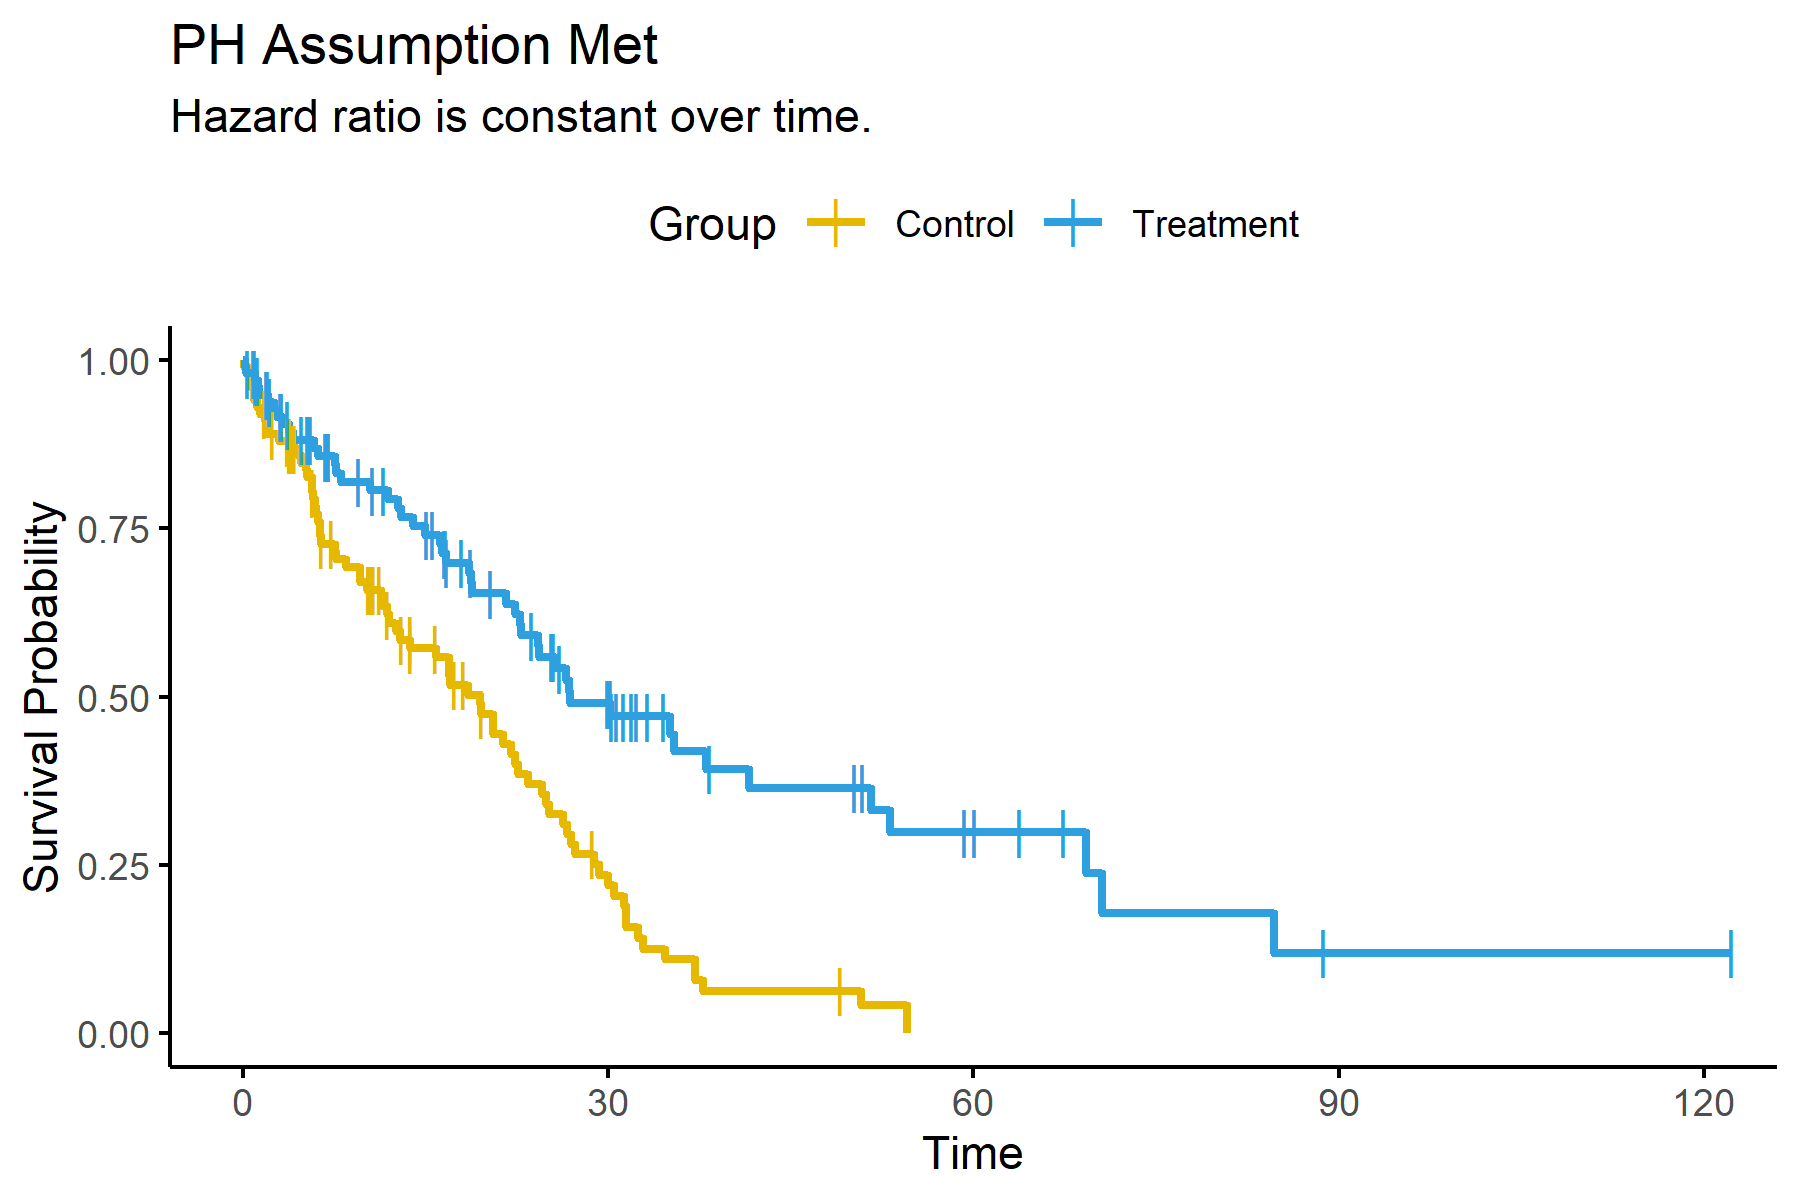
\includegraphics[width=\textwidth]{images/ph_assumption_met.png}
\end{column}
\begin{column}{0.5\textwidth}
    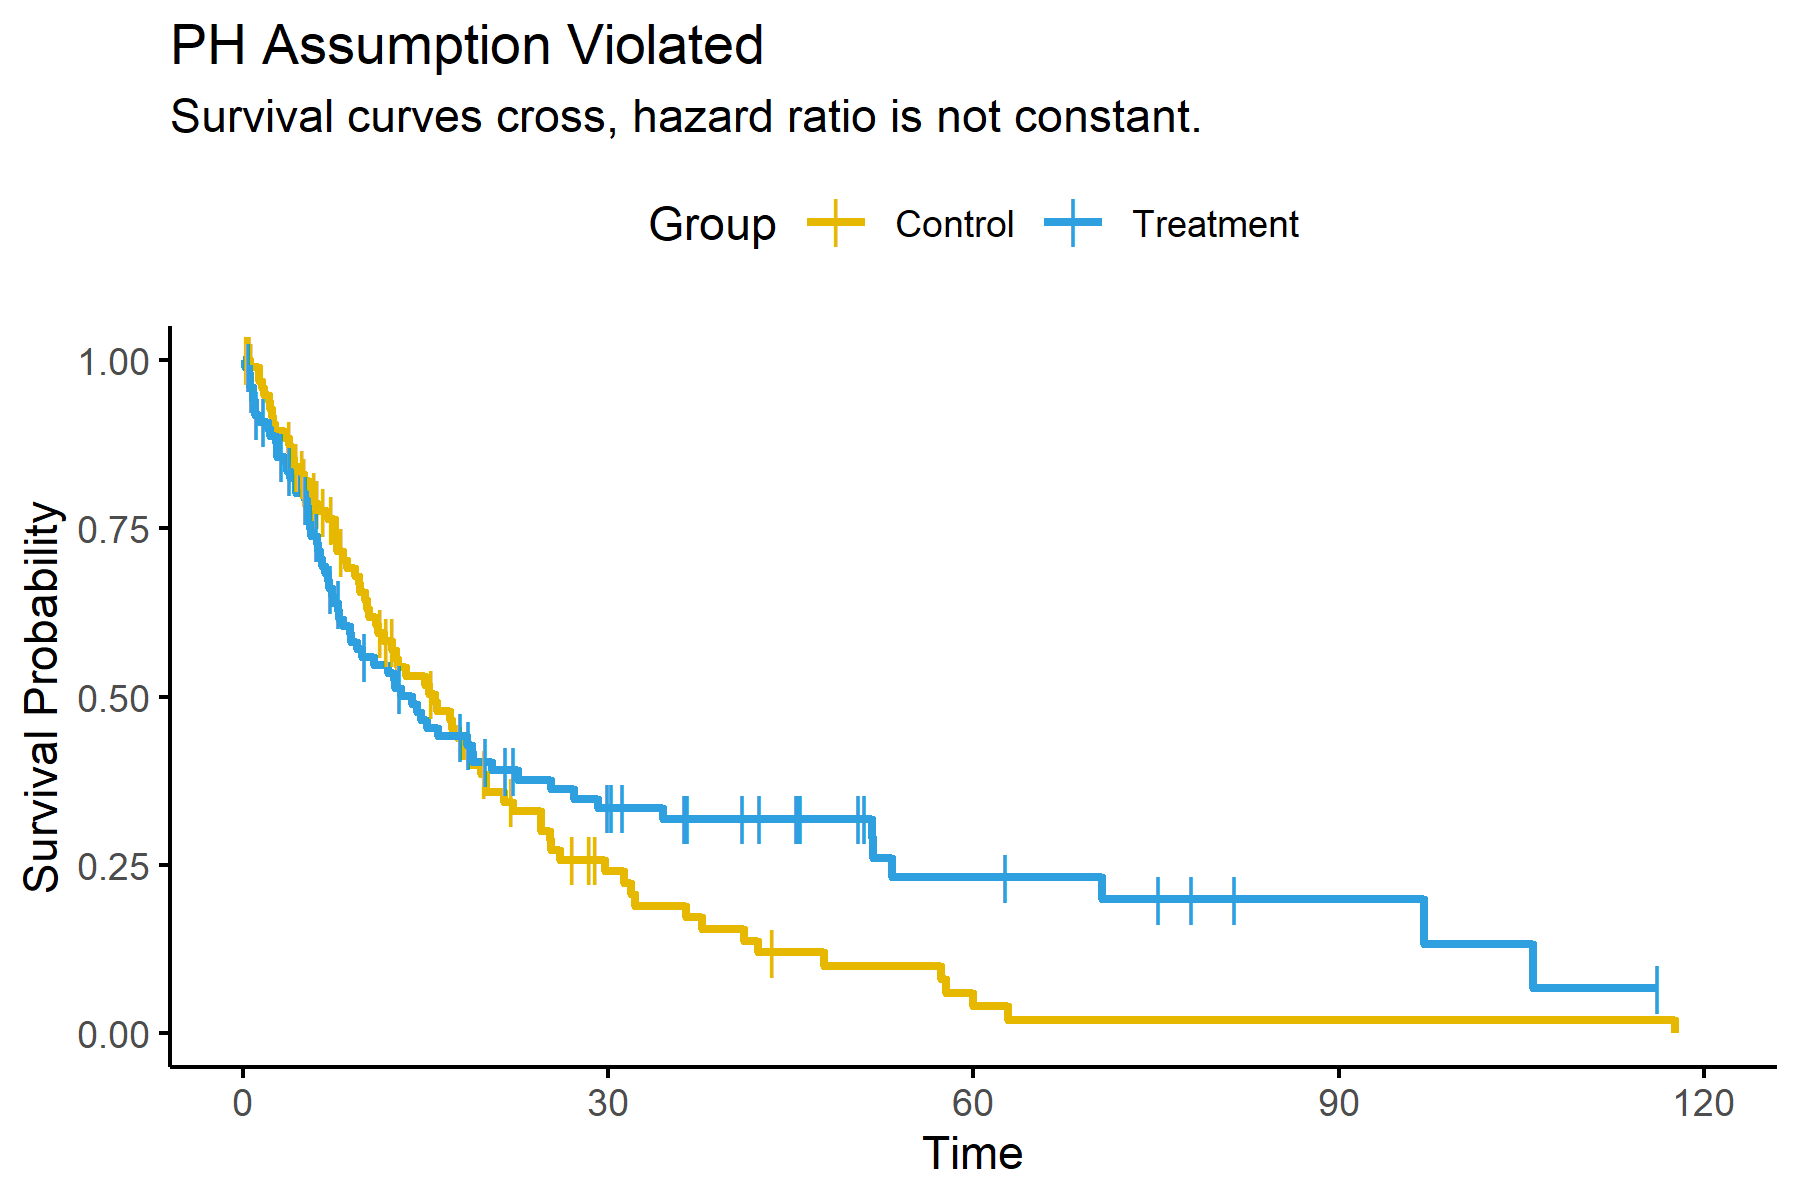
\includegraphics[width=\textwidth]{images/ph_assumption_violated.png}
\end{column}
\end{columns}
\end{frame}

% Frame 5: Problems with the Hazard Ratio
\begin{frame}
\frametitle{Problems with the Hazard Ratio}
\begin{enumerate}
    \item \textbf{The PH Assumption is Often Violated}
    \begin{itemize}
        \item Modern therapies (e.g., immunotherapies) often have \textbf{delayed effects}.
        \item Treatment benefits may \textbf{wear off} over time.
        \item This leads to \textbf{crossing survival curves}, a clear violation of the PH assumption.
    \end{itemize}
    \vspace{1em}
    \item \textbf{Lack of a Clear Causal Interpretation}
    \begin{itemize}
        \item When the PH assumption fails, the single HR value from a Cox model becomes a complex, time-averaged summary.
        \item It loses its clear meaning as a constant relative risk, making it difficult to interpret the true clinical benefit \cite{uno2014}.
    \end{itemize}
\end{enumerate}
\end{frame}

% Frame 6: The Solution: Restricted Mean Survival Time (RMST)
\begin{frame}
\frametitle{The Solution: Restricted Mean Survival Time (RMST)}
\begin{block}{Definition}
The RMST is the average event-free survival time up to a pre-specified time point, $L$. It is the area under the survival curve from 0 to $L$.
$$\mu(L) = E[\min(T, L)] = \int_0^L S(t) dt$$
\end{block}

\begin{block}{Interpretation \& Advantages}
\begin{itemize}
    \item \textbf{Directly Interpretable:} It provides a clear, absolute measure of survival in units of time (e.g., "an average of 3 months of additional survival over 5 years").
    \item \textbf{No Proportional Hazards Assumption:} The RMST is a non-parametric measure, making it a valid and robust choice even when survival curves cross.
    \item \textbf{Clinically Meaningful:} It quantifies the average time gained or lost, which is highly relevant to both clinicians and patients.
\end{itemize}
\end{block}
\end{frame}

% Frame 7: Causal Interpretation of the RMST Difference
\begin{frame}
\frametitle{Causal Interpretation of the RMST Difference}
The treatment effect is quantified as the difference in RMST between the two arms. This is a clear and collapsible causal estimand.

\begin{block}{The Causal Estimand}
$$\Delta(L) = \mu_{\text{treatment}}(L) - \mu_{\text{control}}(L)$$
\end{block}

\textbf{Interpretation:}
\begin{itemize}
    \item $\Delta(L)$ represents the \textbf{average gain in event-free time} attributable to the treatment over the time period $[0, L]$.
    \item This provides a direct answer to the question:
    \\
    \textit{On average, how much longer did patients on the new treatment live without an event during the study period?}
\end{itemize}
\end{frame}

% Frame 8: Causal Interpretation of RMST (Both Scenarios)
\begin{frame}
\frametitle{Causal Interpretation of RMST}
\begin{columns}
\begin{column}{0.5\textwidth}
\begin{block}{PH Met Case}
The RMST provides an intuitive measure of the average survival benefit.
\end{block}
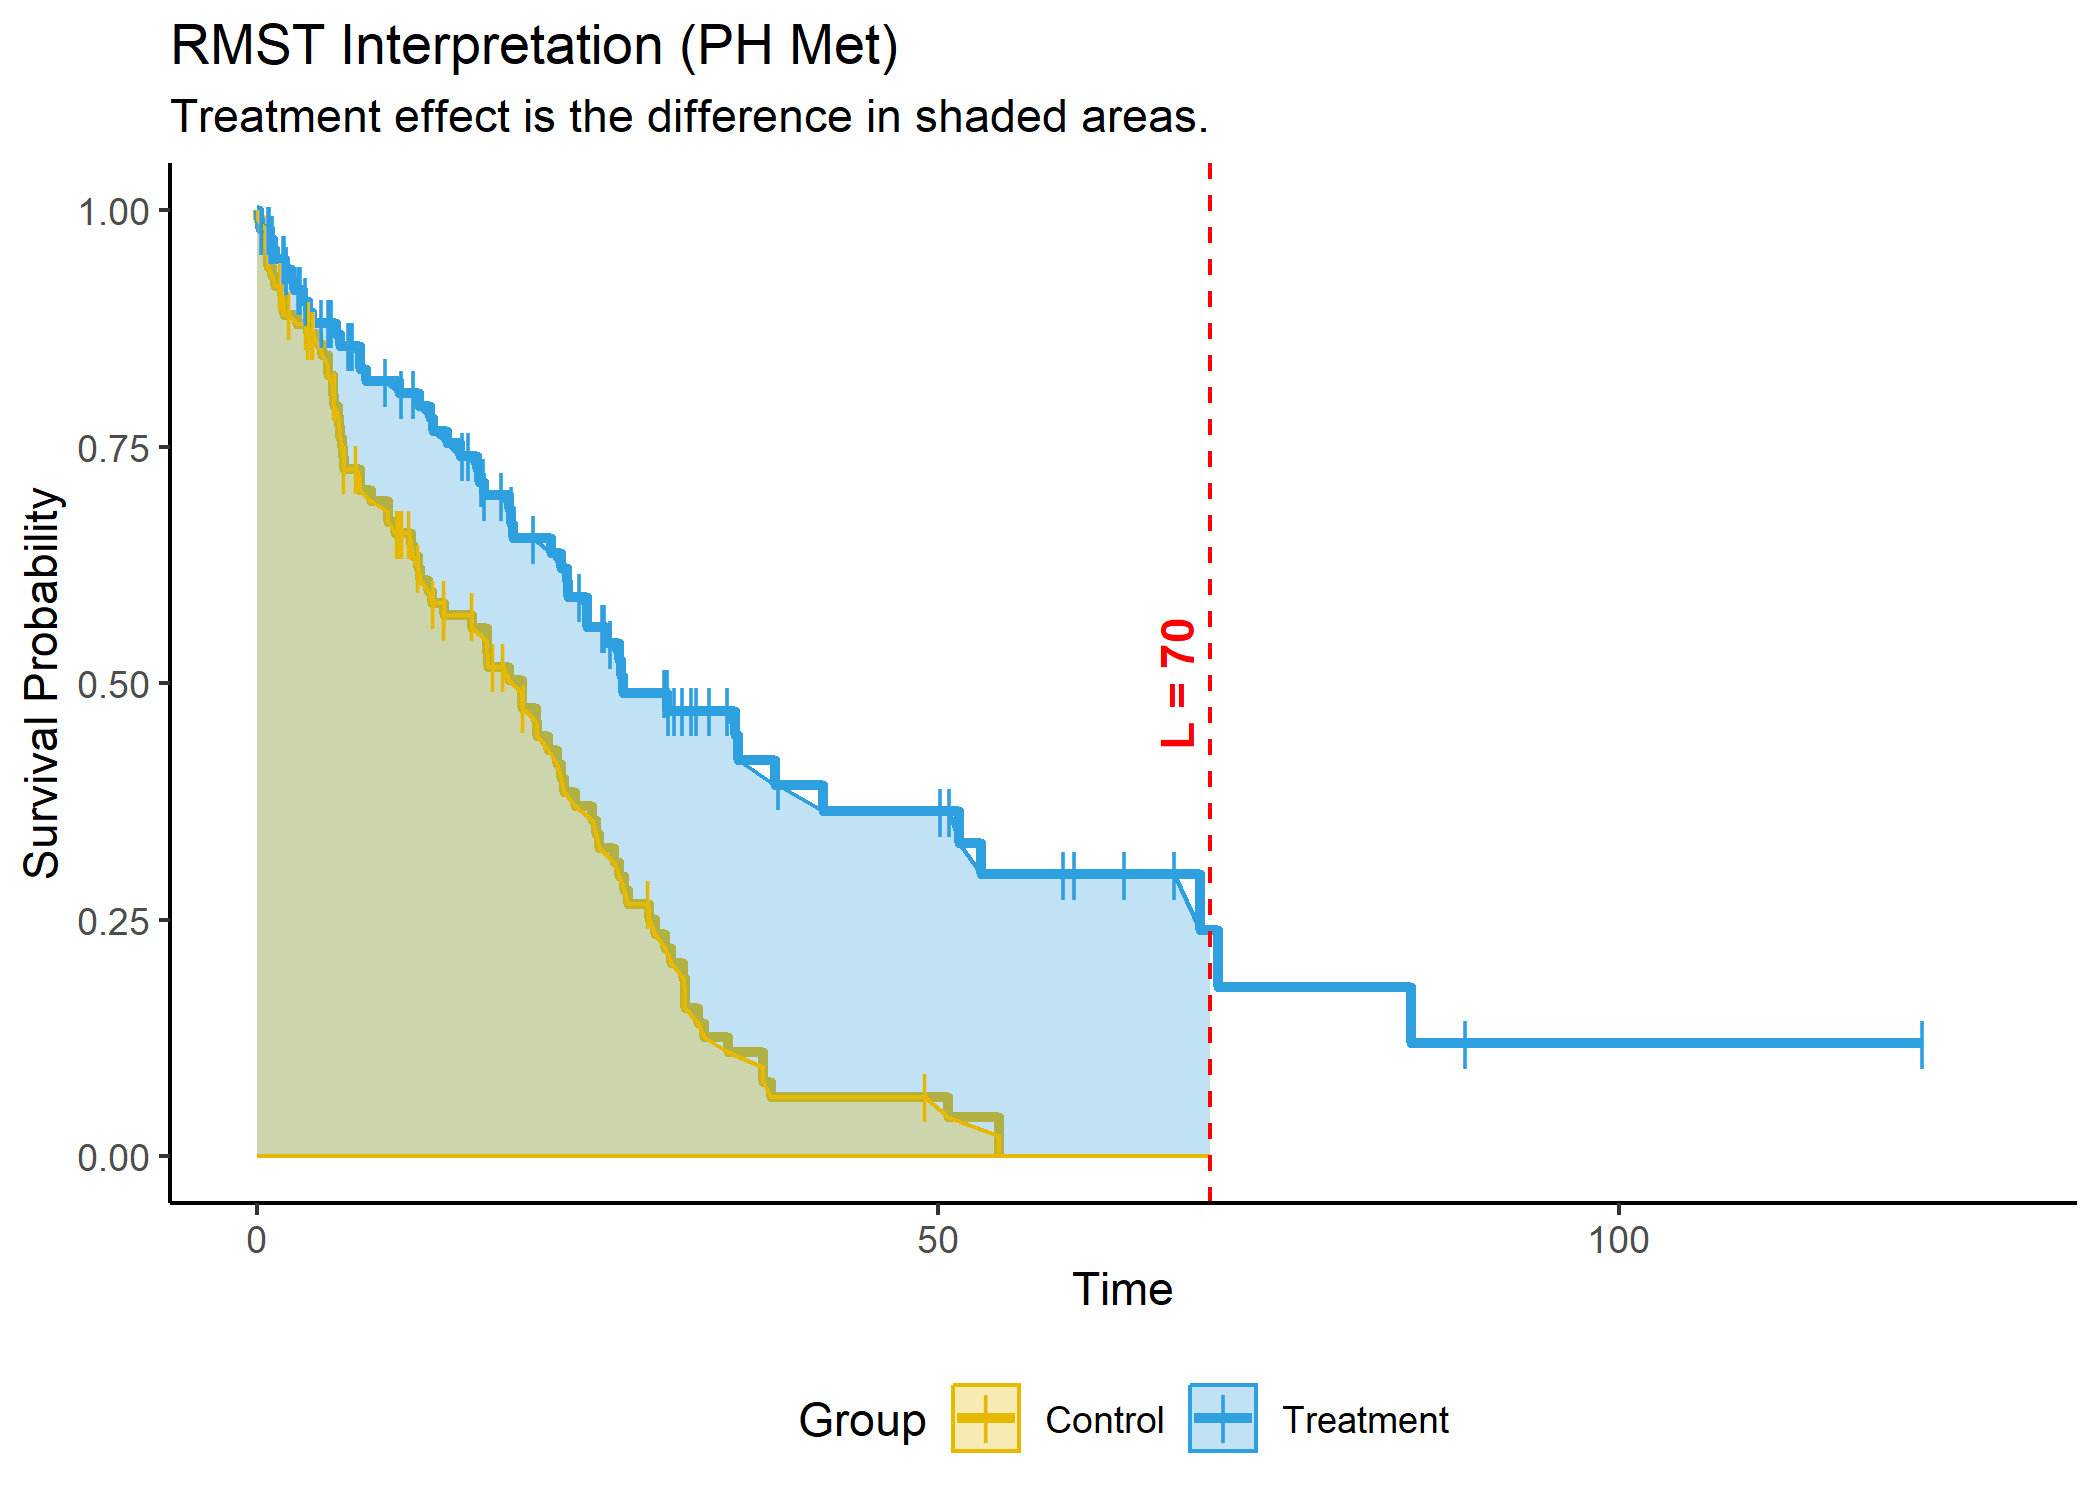
\includegraphics[width=\textwidth, height = 0.8\textwidth]{images/rmst_causal_plot_ph_met.png}
\end{column}
\begin{column}{0.5\textwidth}
\begin{block}{PH Violated Case}
Even with crossing curves, the RMST gives a valid summary of the net effect.
\end{block}
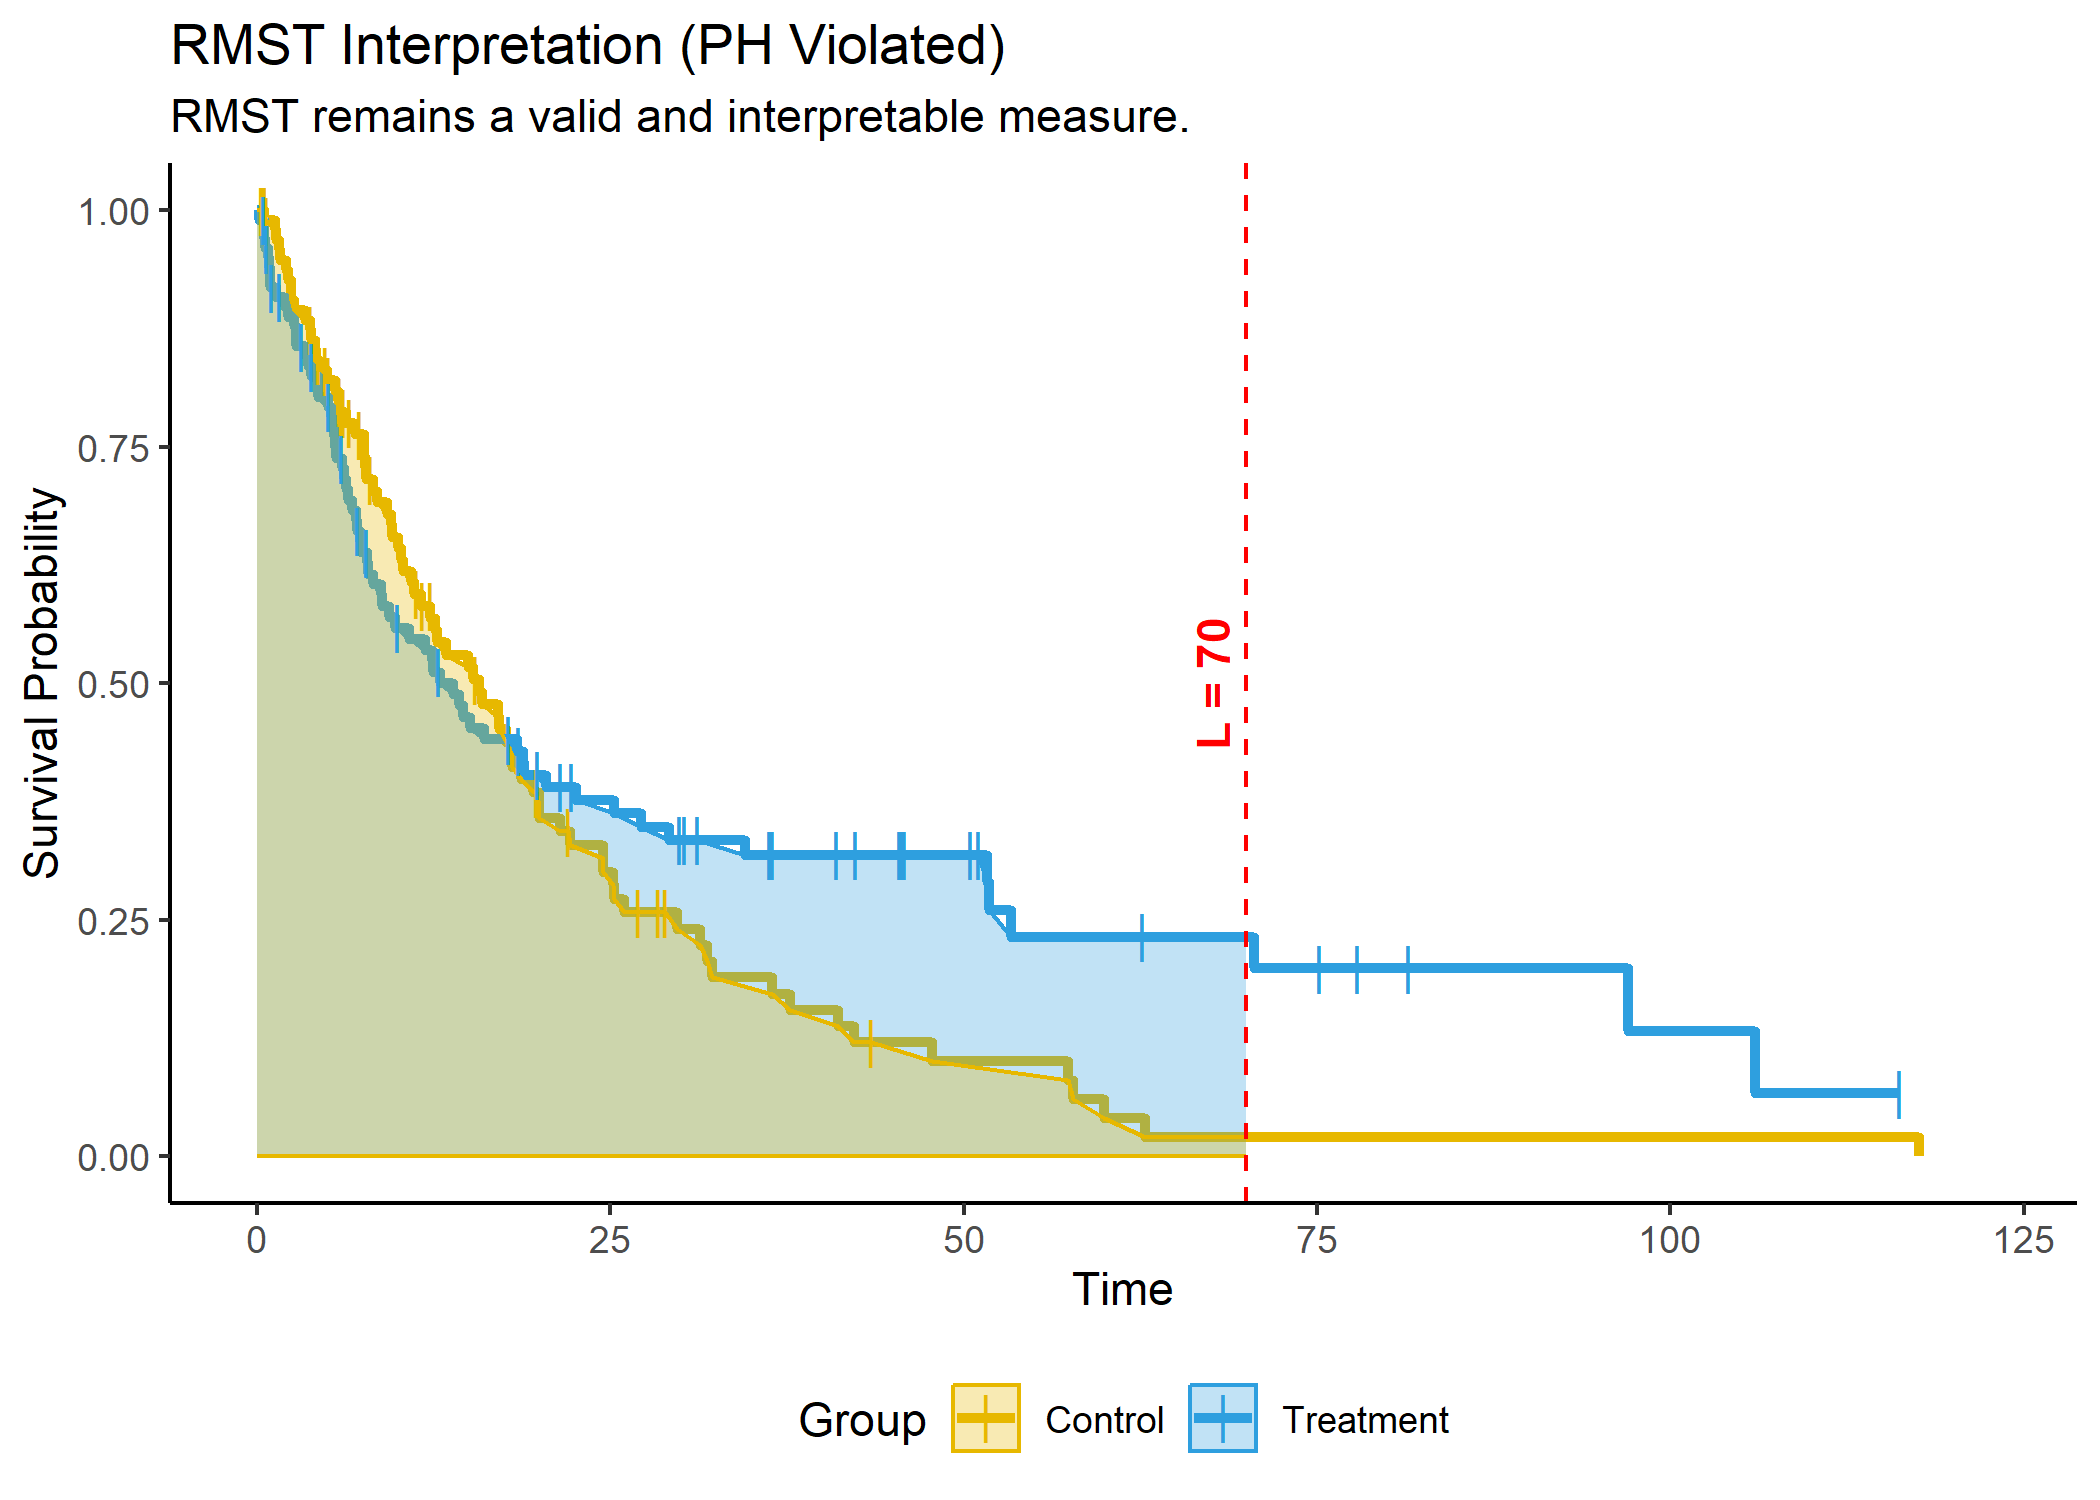
\includegraphics[width=\textwidth, height = 0.8\textwidth]{images/rmst_causal_plot_ph_violated.png}
\end{column}
\end{columns}

\textit{The treatment effect is the difference in area between the two shaded regions.}

\end{frame}

% --- Part 2: The RMSTSS Package: Models & Methods ---
\section{The RMSTSS Package: Models \& Methods}

% Frame 9: Overview of Implemented Models
\begin{frame}
\frametitle{Overview of Implemented Models}
\begin{figure}
    \centering
    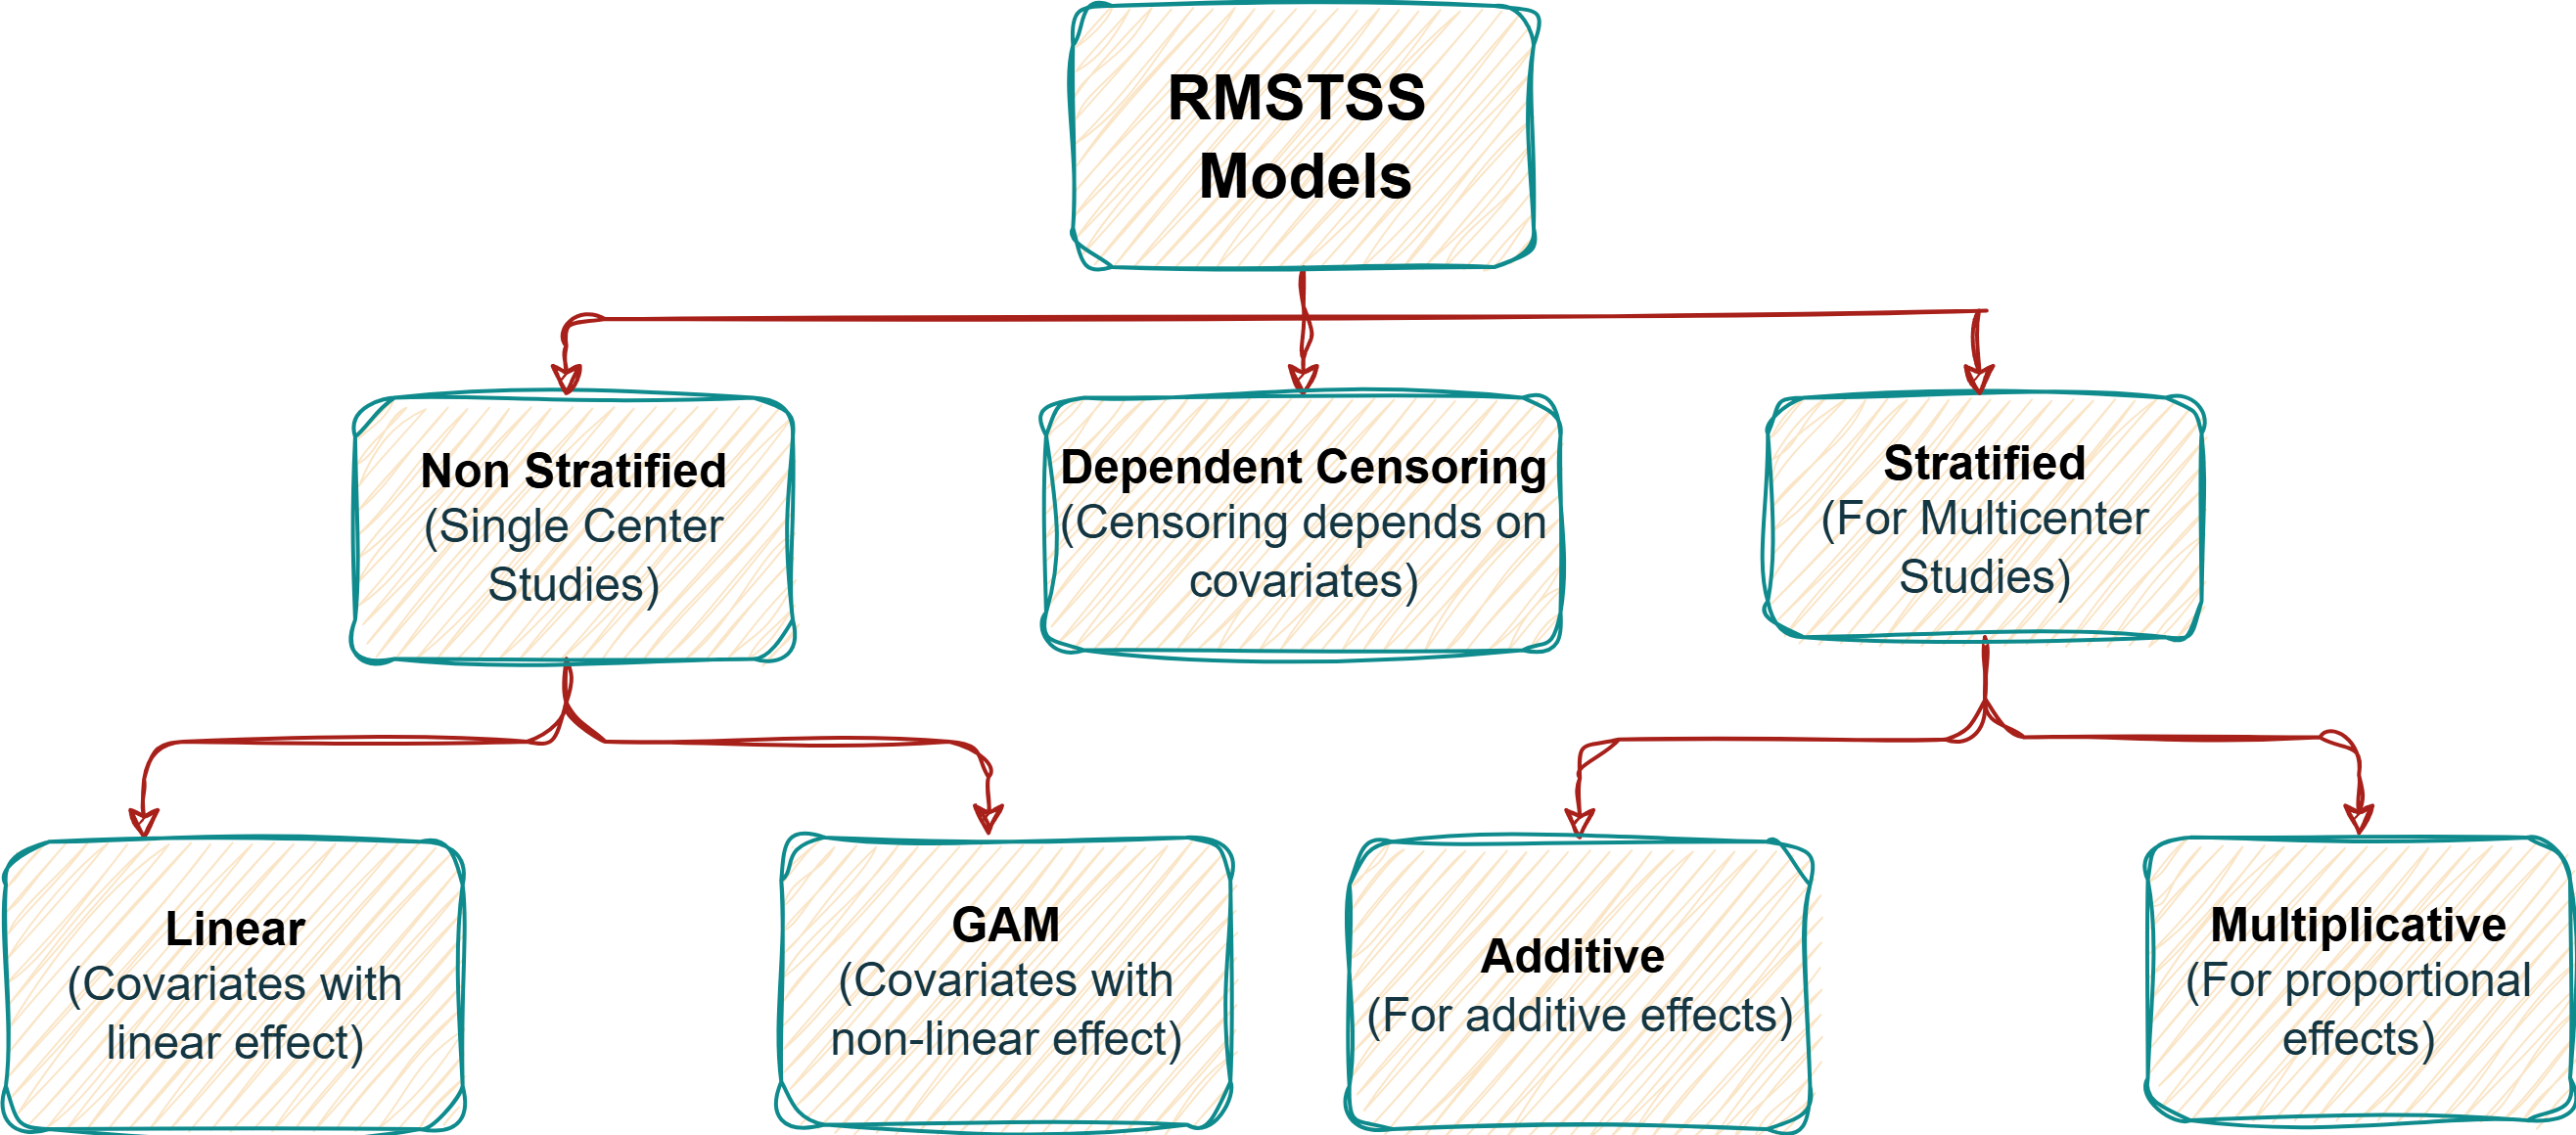
\includegraphics[width=1\linewidth]{images/app-models.png}
\end{figure}
\end{frame}


% --- Part 3: Non-Stratified Models ---

% ---------- Frame 11 ----------
\begin{frame}
\frametitle{Notation for Estimation Slides}

\begin{block}{Observed Data}
For subject $i=1,\dots,n$:
\begin{itemize}
  \item $T_i$: true event time
  \item $C_i$: censoring time
  \item $Y_i = \min(T_i, C_i)$: observed follow-up time
  \item $\delta_i = \mathbb{1}(T_i \le C_i)$: event indicator
  \item $A_i \in \{0,1\}$: treatment group (1 = treatment, 0 = control)
  \item $Z_i$: baseline covariates
\end{itemize}
\end{block}

\begin{block}{Restricted Mean Survival Time}
At restriction time $L$, the RMST is
\[
\mu(L) = E[\min(T,L)] = \int_0^L S(t)\,dt.
\]
\end{block}

\end{frame}

% ---------- Frame 12 ----------
\begin{frame}
\frametitle{Linear Model for RMST}

\begin{block}{Model}
We assume the conditional mean RMST is linear in treatment and covariates:
\[
E[\min(T_i,L) \mid A_i, Z_i] = \beta_0 + \beta_A A_i + \beta_Z^\top Z_i.
\]
\end{block}

\begin{block}{Target Estimand}
\[
\beta_A = \text{adjusted difference in RMST between treatment arms}.
\]
\end{block}


\begin{block}{Problem}
We cannot directly regress $Y_i$ on $(A_i,Z_i)$, because:
\begin{itemize}
  \item If $\delta_i=0$, $Y_i$ is censored, not equal to $T_i$.
  \item $\min(T_i,L)$ is only partially observed when censoring occurs before $L$.
\end{itemize}
\end{block}

\begin{block}{Solution}
We adjust for censoring using \textbf{Inverse Probability of Censoring Weights (IPCW)}.
\end{block}

\end{frame}

% ---------- Frame 14 ----------
\begin{frame}
\frametitle{Estimation with IPCW}

\begin{block}{Censoring Distribution}
Let $G(t) = P(C_i > t)$ be the survival function of censoring time.  
We estimate $\widehat{G}(t)$ using Kaplan–Meier (or Cox if $G$ depends on covariates).
\end{block}

\begin{block}{Weights}
Each subject receives weight
\[
w_i = \frac{\delta_i}{\widehat{G}(Y_i)}.
\]
\end{block}

\begin{block}{Weighted Least Squares}
Estimate $\beta$ by minimizing
\[
\widehat{\beta} = \arg\min_\beta \sum_{i=1}^n w_i \Big\{ Y_i - (\beta_0 + \beta_A A_i + \beta_Z^\top Z_i)\Big\}^2.
\]
\end{block}

\end{frame}

% ---------- Frame 15 ----------
\begin{frame}
\frametitle{Pseudo-Observations for RMST}

\begin{block}{Idea}
Instead of weighted regression, we create \textbf{pseudo-observations} for each subject.
\end{block}

\begin{block}{Definition}
Let $\widehat{\mu}(L)$ = RMST estimate from full sample,  
$\widehat{\mu}^{(-i)}(L)$ = RMST estimate with subject $i$ removed.  
Then
\[
\text{pseudo}_i(L) = n \cdot \widehat{\mu}(L) - (n-1)\cdot \widehat{\mu}^{(-i)}(L).
\]
\end{block}

\begin{block}{Property}
$E[\text{pseudo}_i(L)] = E[\min(T_i,L)]$.  
Thus pseudo-observations can be treated as uncensored outcomes.
\end{block}

\end{frame}

% ---------- Frame 16 ----------
\begin{frame}
\frametitle{Semiparametric GAM Model}

\begin{block}{Model}
We fit a Generalized Additive Model (GAM) to pseudo-observations:
\[
E[\text{pseudo}_i(L)] = \beta_0 + \beta_A A_i + \sum_{k=1}^q f_k(Z_{ik}),
\]
where $f_k(\cdot)$ are smooth spline functions.
\end{block}

\begin{block}{Estimand}
$\beta_A$: adjusted difference in RMST,  
allowing for non-linear effects of covariates.
\end{block}

\end{frame}

% ---------- Frame 18 ----------
\begin{frame}
\frametitle{Stratified Models}

\begin{block}{Additive Model}
Assume each stratum $j$ has its own baseline $\alpha_j$, with a common treatment effect:
\[
E[\min(T_i,L) \mid A_i, S_i=j] = \alpha_j + \beta_A A_i + \beta_Z^\top Z_i.
\]
Interpretation: $\beta_A$ is the constant added survival time across strata.
\end{block}

\begin{block}{Multiplicative Model}
Assume proportional treatment effect across strata:
\[
E[\min(T_i,L) \mid A_i, S_i=j] = \mu_{0j}(L) \cdot \exp(\beta_A A_i + \beta_Z^\top Z_i).
\]
Interpretation: $\exp(\beta_A)$ is the RMST ratio (treatment vs. control), common across strata.
\end{block}

\end{frame}

% ---------- Frame 17 ----------
\begin{frame}
\frametitle{Dependent Censoring}

\begin{block}{Problem}
If censoring depends on covariates, a single $\widehat{G}(t)$ is biased.
\end{block}

\begin{block}{Solution: Cause-Specific Models}
For $K$ censoring causes, fit cause-specific hazards $\lambda_{Ck}(t \mid Z)$ and cumulative hazards $\Lambda_{Ck}(t \mid Z)$.  
Then
\[
\widehat{G}(t \mid Z) = \exp\!\Big(-\sum_{k=1}^K \widehat{\Lambda}_{Ck}(t \mid Z)\Big).
\]
\end{block}

\begin{block}{IPCW with Dependent Censoring}
Use $\widehat{G}(t \mid Z)$ in the IPCW weights.
\end{block}

\end{frame}

% --- Part 6: Software & Conclusion ---
% ---------- Frame 19 ----------
\begin{frame}
\frametitle{Core Computational Approaches for Power and Sample Size}

\begin{block}{Analytical Approach}
Uses asymptotic variance of the estimated treatment effect:
\[
\text{Power} = 
\Phi\!\left( 
\frac{|\widehat{\beta}_A|}{\widehat{\sigma}_{\beta_A}/\sqrt{n}} - z_{1-\alpha/2}
\right),
\]
where $\widehat{\sigma}_{\beta_A}$ is the estimated standard error and $\Phi$ is the standard normal CDF.
\end{block}

\begin{block}{Bootstrap Approach}
Simulation-based resampling from pilot data:
\[
\text{Power} =
\frac{\#\{\text{replicates with $p$-value} < \alpha\}}{B},
\]
where $B$ = number of bootstrap replicates.
\end{block}

\end{frame}

% ---------- Frame 20 ----------
\begin{frame}
\frametitle{Package Functionality \& Naming Convention}

Functions follow a consistent naming format:
\[
\texttt{model.goal.method()}
\]

\begin{itemize}
  \item \textbf{Model:} \texttt{linear}, \texttt{GAM}, \texttt{DC}, \texttt{additive}, \texttt{MS}
  \item \textbf{Goal:} \texttt{power} (estimate power) or \texttt{ss} (sample size for target power)
  \item \textbf{Method:} \texttt{analytical} or \texttt{boot}
\end{itemize}

\begin{block}{Example}
\texttt{MS.ss.boot()}  
$\Rightarrow$ Sample size calculation for Multiplicative Stratified model, via bootstrap.
\end{block}

\end{frame}

% ---------- Frame 21 ----------
\begin{frame}[fragile]
\frametitle{Worked Example: Additive Stratified Model}

\begin{block}{Scenario}
Multi-center trial from \texttt{colon} dataset.  
Goal: Required sample size per stratum to achieve $80\%$ power, truncation time $L = 1825$ days (5 years).
\end{block}

\begin{block}{R Code}
\begin{verbatim}
library(survival)
library(RMSTSS)

# Prepare pilot data
colon_death <- colon[colon$etype == 2, ] %>% na.omit()
colon_death$arm <- ifelse(colon_death$rx == "Obs", 0, 1)
colon_death$strata <- factor(colon_death$extent)

# Sample size calculation
ss_results <- additive.ss.analytical(
  pilot_data = colon_death,
  time_var   = "time",
  status_var = "status",
  arm_var    = "arm",
  strata_var = "strata",
  target_power = 0.80,
  L = 1825
)

print(ss_results$results_data)
\end{verbatim}
\end{block}

\end{frame}

% ---------- Frame 22 ----------
\begin{frame}[fragile]
\frametitle{Worked Example: Bootstrap Sample Size Calculation}

\begin{block}{Scenario}
Same multi-center trial from the \texttt{colon} dataset.  
Goal: Required sample size per stratum to achieve $80\%$ power at $L = 1825$ days,  
using the \textbf{bootstrap method}.
\end{block}

\begin{block}{R Code}
\scriptsize
\begin{verbatim}
# Sample size calculation using bootstrap method
ss_boot <- additive.ss.boot(
  pilot_data   = colon_death,
  time_var     = "time",
  status_var   = "status",
  arm_var      = "arm",
  strata_var   = "strata",
  target_power = 0.80,
  L            = 1825,
  n_boot       = 500   # number of bootstrap replicates
)

print(ss_boot$results_data)
\end{verbatim}
\end{block}

\begin{block}{Interpretation}
The bootstrap approach directly simulates variability from pilot data,  
providing a more robust estimate of sample size under complex censoring patterns.
\end{block}
\end{frame}


% ---------- Frame 22 ----------
\begin{frame}
\frametitle{The \texttt{RMSTSS} Shiny Application}

\begin{block}{Key Features}
\begin{itemize}
  \item Upload pilot data in \texttt{.csv} format
  \item Map columns (time, status, treatment, strata) via dropdown menus
  \item Select model (\texttt{linear}, \texttt{GAM}, \texttt{additive}, \texttt{MS}, \texttt{DC})
  \item Choose goal (\texttt{power} or \texttt{ss}) and method (\texttt{analytical} or \texttt{boot})
  \item Interactive outputs: survival curves, power curves
  \item Export analysis reports in pdf
\end{itemize}
\end{block}

\end{frame}

% ---------- Frame 23 ----------
\begin{frame}
\frametitle{Application Interface}
\begin{figure}
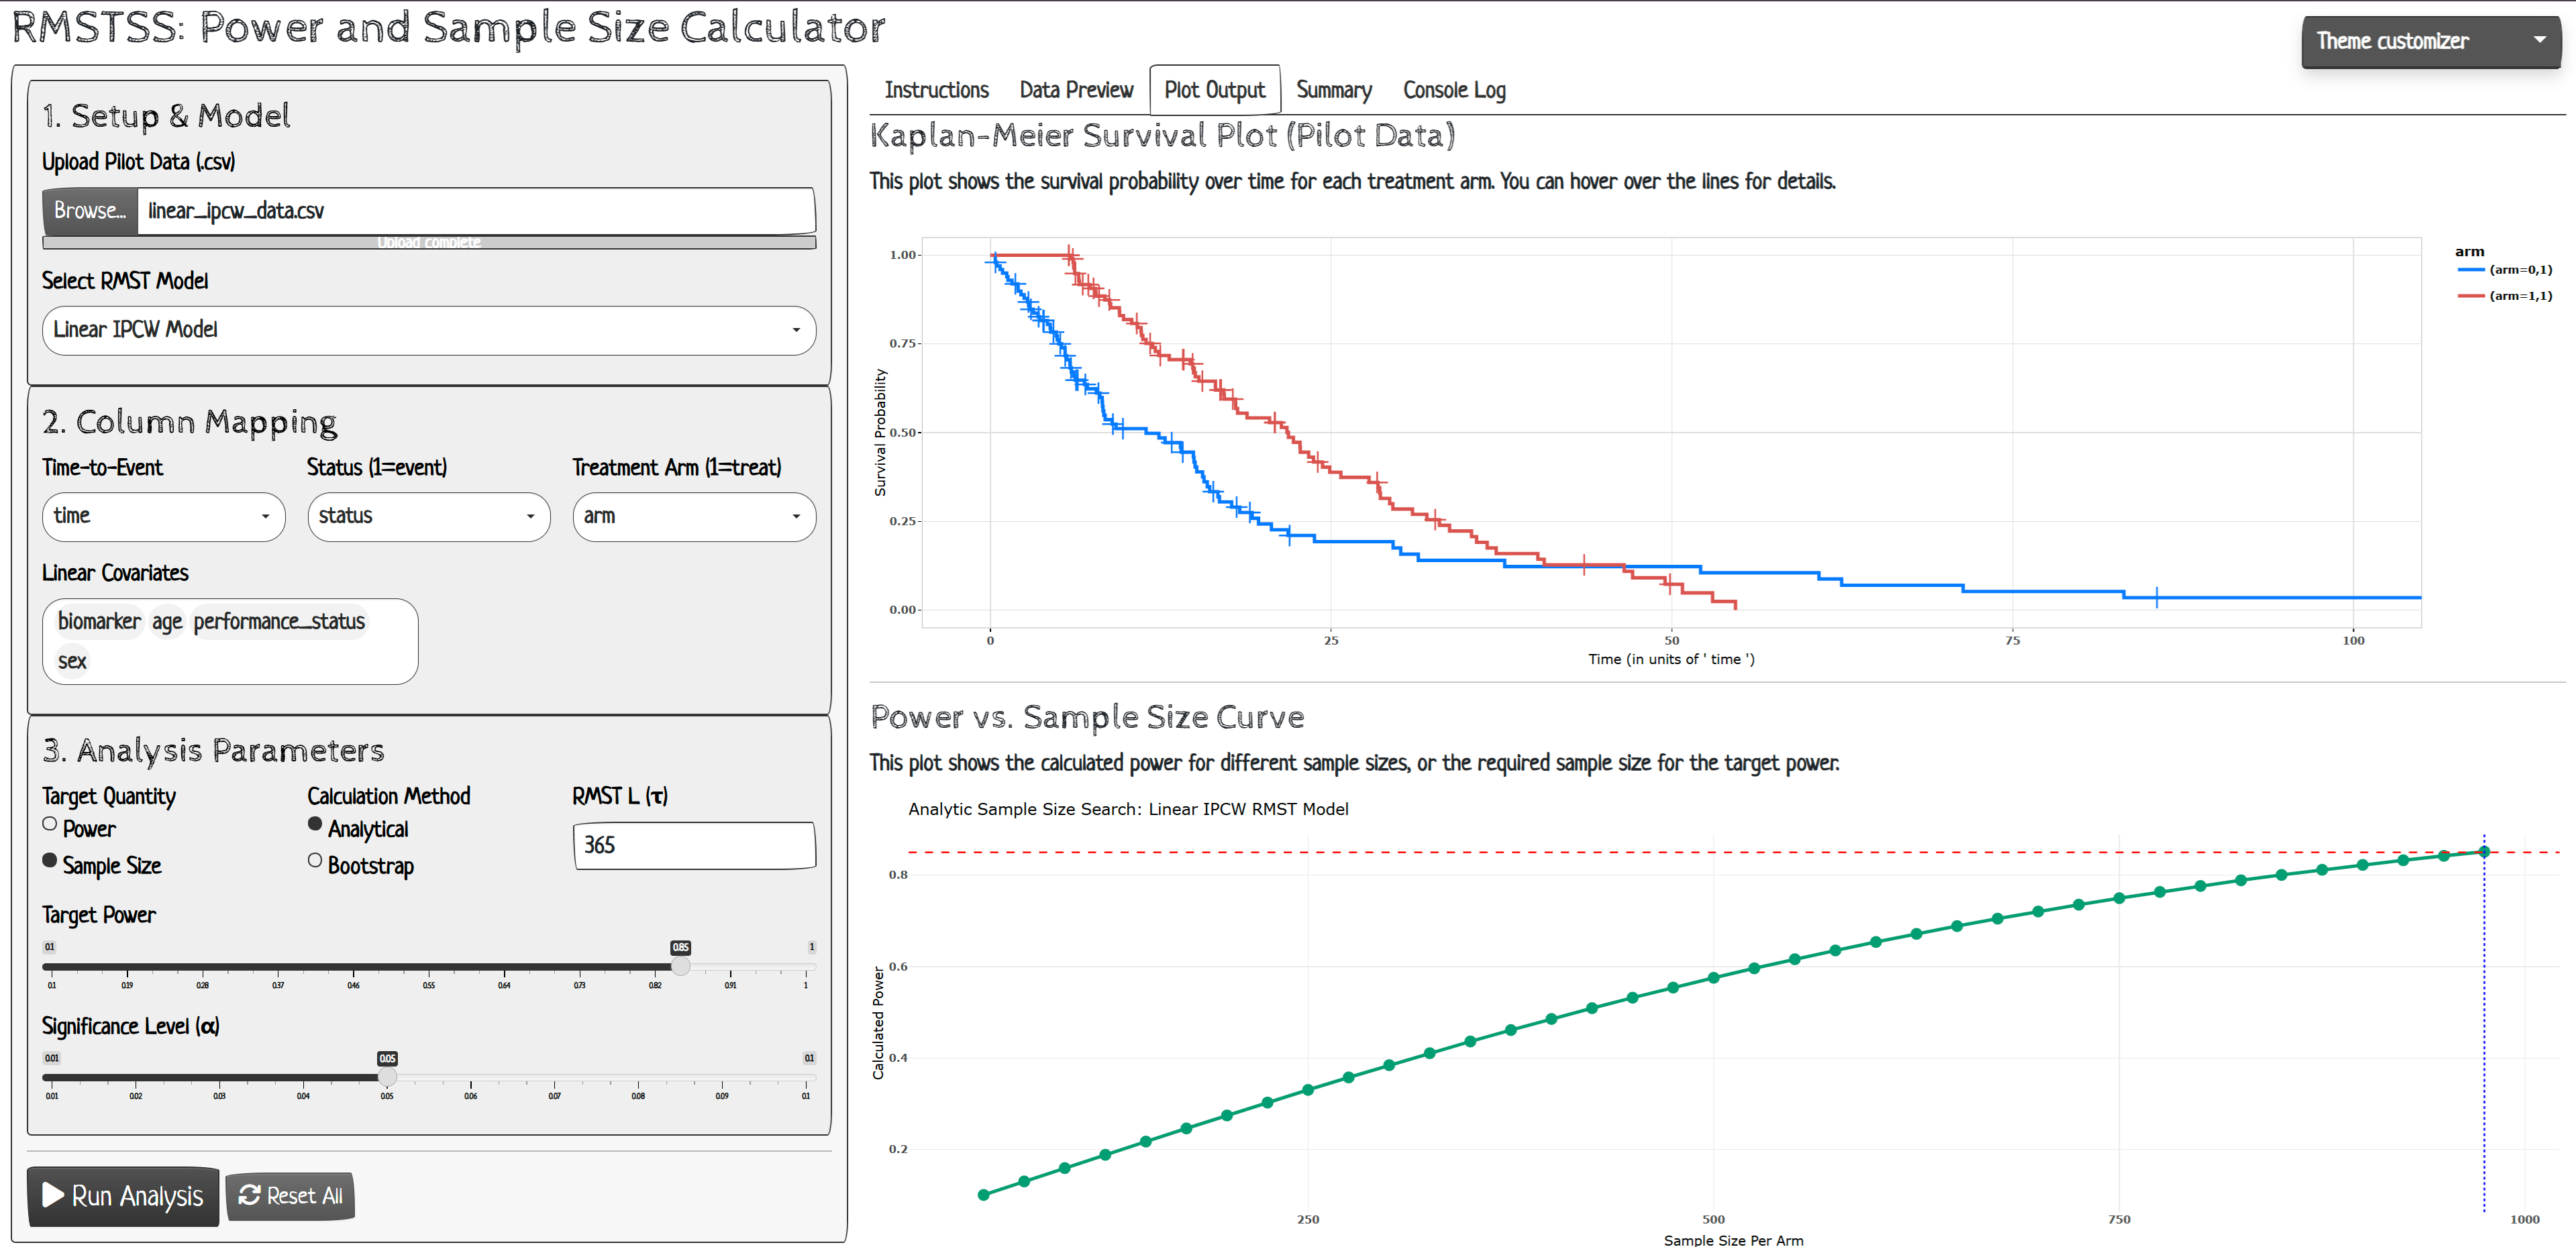
\includegraphics[width=\textwidth]{images/app-ss.png}
\caption{Analysis panel of the Shiny application: model selection and result visualization.}
\end{figure}
\end{frame}

% ---------- Frame 24 ----------
\begin{frame}
\frametitle{Conclusion \& Future Aims}

\begin{block}{Conclusion}
\begin{itemize}
  \item \textbf{Statistically Rigorous:} Implements linear, GAM, dependent censoring, and stratified RMST models
  \item \textbf{Causally Interpretable:} Treatment effect $\beta_A$ (difference) or $\exp(\beta_A)$ (ratio)
  \item \textbf{Practical:} Available as both an R package and a Shiny web app
\end{itemize}
\end{block}

\begin{block}{Future Aims}
\begin{itemize}
  \item Extend RMSTSS to handle \textbf{time-varying treatments} and adaptive designs
  \item Incorporate \textbf{Bayesian approaches} for RMST-based trial planning
  \item Develop modules for \textbf{multi-arm and platform trials}
  \item Improve \textbf{Shiny app interactivity} with dynamic simulation dashboards
\end{itemize}
\end{block}
\end{frame}

% Frame 25: References
\begin{frame}[allowframebreaks]
\frametitle{References}
\scriptsize
\bibliographystyle{plainnat}
\bibliography{references}
\end{frame}

% Frame 26: Access & Acknowledgments
\begin{frame}
\frametitle{Access \& Acknowledgments}
\begin{columns}[T]
\begin{column}{0.5\textwidth}
\scriptsize
    \textbf{Acknowledgments}
 \begin{itemize}
        \item Grateful appreciation to Dr.\ Yuan Zhang (UTHSC) for mentorship
        \item Special thanks to Dr.\ Gregory Farage and Dr.\ Saunak Sen (UTHSC) for their guidance and support
        \item Support provided by UTHSC BERD (Biostatistics, Epidemiology, and Research Design)
        \item Research funded by NSF Grant No.\ 2220726
    \end{itemize}
\vfill
\begin{center}
\Huge{\textbf{Questions?}}
\end{center}
\end{column}
    \begin{column}{0.5\textwidth}
    \scriptsize
        \centering
        \textbf{Scan for Web App} \\
        \qrcode[height=3cm]{https://arnab96.shinyapps.io/uthsc-app/}
        \vspace{2em}
        \\
        \textbf{Scan for R Package} \\
        \qrcode[height=3cm]{https://uthsc-zhang.github.io/RMSTSS-Package/}
    \end{column}
\end{columns}
\end{frame}

\end{document}
